\documentclass[a1,portrait]{a0poster}

%\usepackage{revtex4}
\usepackage{multicol} % This is so we can have multiple columns of text side-by-side
\columnsep=30pt % This is the amount of white space between the columns in the poster
\columnseprule=1pt % This is the thickness of the black line between the columns in the poster
\usepackage[usenames,dvipsnames]{xcolor}
\definecolor{1}{RGB}{66,92,138}
\definecolor{2}{RGB}{60,83,122}
\definecolor{3}{RGB}{51,102,102}
%\usepackage[svgnames]{xcolor} % Specify colors by their 'svgnames', for a full list of all colors available see here: http://www.latextemplates.com/svgnames-colors
\usepackage{times} % Use the times font
%\usepackage{palatino} % Uncomment to use the Palatino font
\usepackage{graphicx} % Required for including images
\graphicspath{{figures/}} % Location of the graphics files
\usepackage{booktabs} % Top and bottom rules for table
\usepackage[font=small,labelfont=bf]{caption} % Required for specifying captions to tables and figures
\usepackage{amsfonts, amsmath, amsthm, amssymb} % For math fonts, symbols and environments
\usepackage{wrapfig} 
\usepackage{natbib}
\usepackage[utf8]{inputenc}
\let\babellll\lll
\let\lll\relax
\begin{document}

\begin{minipage}[b]{0.6\linewidth}
\Huge \color{2} {The search of new Higgs boson} \color{Black}\\ % Title
%\Huge\textit{}
\\[1cm] % Subtitle
\large \textbf{Marta Sawko and Grzegorz Czelusta}
\\[0.5cm] % Author(s)
University of Wrocław
\\[0.4cm] % University/organization
\end{minipage}
%\vspace{1cm} % A bit of extra whitespace between the header and poster content

%----------------------------------------------------------------------------------------

\begin{multicols}{2} % This is how many columns your poster will be broken into, a portrait poster is generally split into 2 columns
\color{3} % SaddleBrown color for the introduction

\section*{Introduction}
The Standard Model of particle physics is one of the most thoroughly verified theories in science.
The drawbacks of the Standard Model (SM) motivate search for beyond
Standard Model physics. The most popular theory explaining spontaneously-broken supersymmetry (SUSY) is called
the Minimal Supersymmetric Standard Model. It assumes that every particle has its superpartner and 
predicts the existence of the five Higgs bosons.
\textbf{ATLAS} experiment, which is run in Large Hadron Collider at CERN in Switzerland, studies the consequences of
Standard Model
and the nature of beyond Standard Model physics. The beams of protons are accelerated, collide and later are being 
examined in the detector.
We conducted our analysis using \textbf{ROOT}, which is a C++ library built by CERN.
The study focuses on eight types of probes in terms of signal masses which were hypothetical boson signals. 
We examine the final state of H/A boson decay --- one pair of $b\overline{b}$ and one $b$-quark.



 \begin{center}
   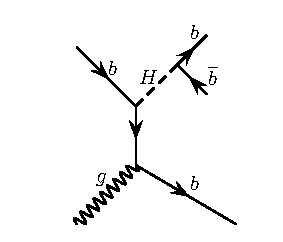
\includegraphics[width=0.20\textwidth]{./feynman.pdf}
 \end{center}
 
\color{Black} % DarkSlateGray color for the rest of the content

\section*{Application of Monte Carlo}
During our research we relied on Monte Carlo method. 
Though events generated by Monte Carlo do not faithfully reflect reality,
they accurately reproduce signal to the background ratio.
The Monte Carlo events were generated way before the real data, according to the detector 
limitations and to the theoretical expectations from the Standard Model. 
Future work will comprise a comparison with the real data.


\section*{The Method}

\subsection*{Cuts and trigger}
The analysis requires appling data reduction techniques during and after gathering data. The first
stage of data selection, run while collecting the data, is the \textbf{trigger} --- it decides about the event-accaptance 
and, in conssequences, reduces the background. The trigger has its three levels: L1, L2, EF. 
It selects by taking into the consideration things like energy, number
and direction of the jets.\\
Later, we begin offline reduction. It consists of specyfic \textbf{cuts} on some jets due to their 
transverse momentum, angle and $b$-taging. $b$-taging means ascribing events to particular cathegory:
\textit{bbb}(strongest demand about existance of third $b$-quark), \textit{bbloose}(less rigorous requirement concerning 
third $b$-quark, smaller likelihood that it will be found), \textit{bbanti}(the smallest probability [..]).

\subsection*{The separation}
In order to better separate the signal and the background, we change the variables as follows. 
We want to define new $m_{bb}'$. We will use the eigenvector $\boldsymbol{v_{extr}}$ with respect to extreme eigenvalue of the following matrix:
\begin{equation}
 \sum_{events} \left(
		    \begin{array}{ccc}
                      m_{bb}m_{bb} & m_{bb}p_{T1} & m_{bb}p_{T2}\\
                      m_{bb}p_{T1} & p_{T1}p_{T1} & p_{T1}p_{T2}\\
                      m_{bb}p_{T2} & p_{T1}p_{T2} & p_{T2}p_{T2}\\
                     \end{array}
                \right).
\end{equation}
We define
\begin{equation}
 m_{bb}'
 =
 \left(
 \begin{array}{ccc}
       m_{bb} & p_{T1} & p_{T2} 
       \end{array}
\right) \cdot \boldsymbol{v_{extr}}.
\end{equation}
Let us try to visualize the change of the variables. 



\begin{center}
  \includegraphics[width=0.2\textwidth]{./separacja.eps}
\end{center}

\subsection*{Background estimation}
Using Monte Carlo we can well simulate the ratio of the background in the case of three quarks
with case of two quarks. 
We know that in the case of two $b$-quarks in the final state there is no chance of the occurrence of
the boson. 
Hence, even in real probe we will have only the background. 
The situation might be different in terms of case of our main interest --- that is in three quarks.
The real probe will consist of the background but also the potential signal.
We compare the ratio from the simulation with the ratio from the experiment and search for the 
extra energy.

\begin{center}
  \includegraphics[width=0.2\textwidth]{./ratio.eps}%dofitowany czerwoną, stosunek sy,ulowanych teł
\end{center}

\subsection*{Pseudodata and fit}
We combine simulated signal and simulated background adjusting percentage rate of 
signal, using \textit{RooFit} tool dedicated for ROOT, relaying on background estimation. Fit is applied on every
$b$-tag category simultaneously.\\

While creating the systematics of the errors, we are taking into consideration the mistake of the trigger, momentum, offline
systematics, normalization and transfer factor.
We verify the efficiency of the fit, giving already the mixed data with a certain percentage rate, and checking
what rate and what statistical error the fit will give back.
\begin{center}
  \includegraphics[width=0.2\textwidth]{./statystyka.pdf}
  %x-axis data with a given percent of signal; y-axis what program thinks the percent rage is like
\end{center}

The next step of this work is to substitute the simulated data with the original one.

 %----------------------------------------------------------------------------------------
%	REFERENCES
%----------------------------------------------------------------------------------------

\nocite{doktorat}
\bibliographystyle{plain}
\bibliography{bibliografia} 


\end{multicols}
\end{document}